\section{Appendix} \label{sec: Appendix}
The appendix contains code listening and other large information parts that contain partial or complete relevance to the reports topic. 

\subsection{Lesson Learned} \label{subsec: Lesson Learned}
\subsubsection{Vivado Language Templates} \label{subsubsec: Vivado Language Templates}
Figure \ref{fig: Vivado_LanguageTemplates} shows a handy tool build into Vivado software package that is called Language Templates and it seems to contain most of the verilog syntax.
\begin{figure}[htbp]
	\centering
	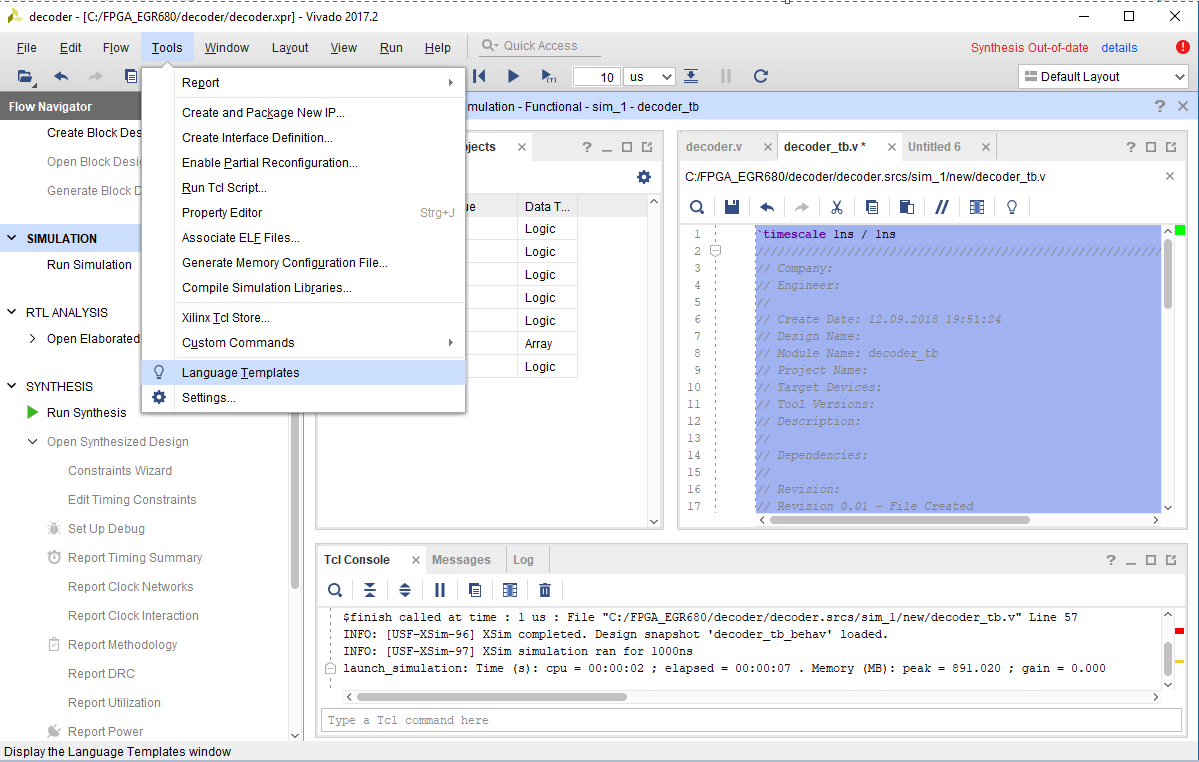
\includegraphics[width=0.6\textwidth]{01_images/Vivado_LanguageTemplates.png}
	\caption{Vivado Language Templates.}
	\label{fig: Vivado_LanguageTemplates}
\end{figure}
\subsubsection{Clock divider not working} \label{subsubsec: Clock divider not working}
Listening \ref{lst: clock divider issue} shows a code snipe out of the clock divider that caused a lot of trouble by preventing the clock divider preventing dividing the clock. It seems that the last statement $clk_out <= clk_out;$ overwrote the statement 
$clk_out <= ~clk_out;$ which results either in an unknown state or an zero on the divided clock instead of the desired toggling clock behavior. 
\begin{lstlisting}[language=verilog,caption={Clock divider issue.},label=lst: clock divider issue]
else
begin

clk_temp <= clk_temp + 1;
if (clk_temp >= 500000) 
//if (clk_temp >= 2) // Used for testbench
begin
clk_out <= ~clk_out; // no clue why this line does not toggle the clk_out
//   if (clk_out == 0) 
//   begin
//   clk_out=1;
//   end 
//   else
//   begin
//   clk_out=0;
//   end
clk_temp <= 0;
end
end // else rst
//clk_out <= clk_out; // could this lane of HDL be causong the problem of the not working clk divider? Yes, it is!!!

\end{lstlisting}

\subsubsection{Implementation Error [Place 30-574] Poor placement for routing between an I/O pin and BUFG} \label{subsubsec: Poor placement for routing between an I/O pin and BUFG}
\href{https://wiki.nus.edu.sg/pages/viewpage.action?pageId=167808307}{Poor placement for routing between an I/O pin and BUFG} is a state where a clk signal is routed to anon clock net or a non clock signal is routed to clock net like a posedge or negedge clk signal.
Now it seems this clock placement error that occurs by implementing the project is somewhat related to the decoder. As the decoder module is commented out of the top level block the error is not there any more. Still the source or what pin shall causing the issue could not be located at first.
The issue was that the in the decoder initialization the clk and rst pin where switched.
